\documentclass[11pt]{article}

\usepackage[english]{babel}
\usepackage{amsmath}
\usepackage{amsfonts}
\usepackage{enumerate}
\usepackage{framed}
\usepackage{graphicx}
\usepackage{textcomp}
\usepackage{listings}
\usepackage{float}
\usepackage{caption}
\usepackage{subcaption}
\oddsidemargin0.5cm
\voffset-2cm
\textwidth15.5cm
\textheight22cm

\lstset{basicstyle=\footnotesize}

\begin{document}
\title{\textsl{GOSM}: Grid Operations Scenario Maker \\ User Manual}
\date{\today}

\maketitle

\section{Introduction}
This document explains the proper usage of the programs associated with scenario creation software in the Python package \texttt{prescient\_gosm}. 
The acronym \textit{GOSM} stands for \textit{Grid Operations Scenario Maker}. \textit{GOSM} consists of various scripts for the computation 
and evaluation of (generally probabilistic) scenarios related to the forecasting of renewable energy production. These scripts include 
\texttt{preprocessor.py}, \texttt{scenario\_creator.py}, \texttt{populator.py}, and \texttt{horse\_racer.py}. The \texttt{preprocessor.py} script
prepares input   for the scenario creation process. The \texttt{scenario\_creator.py} script creates scenarios for a single day from 
one or more sources of uncertainty. The \texttt{populator.py} script is a barebones wrapper of the \texttt{scenario\_creator.py} script, and
offers the additional feature to loop over ranges of dates and produce scenarios for multiple days. Finally, the \texttt{horse\_racer.py} script
uses the \texttt{populator.py} script to create scenarios and then executes the simulator  to produce some 
relevant discrimination statistics concerning different methods for creating and evaluating scenarios.

\section{Installation}

\subsection{Installing \texttt{prescient\_gosm}}
You will obtain the code either from a zip file or by issuing a \texttt{git clone} command. You probably also need to get statdist and run setup.py for it.

Upon downloading the code, you will find the all scripts mentioned in this document in the directory \texttt{<Install Dir>/prescient\_gosm} which will be hereafter referred to as \texttt{\$PRESCIENT}.

You will need to install a collection of other programs to ensure that the scripts will run properly. These programs include \textit{python} of course, as well as a collection of other python modules (mainly \textit{pyomo} and the modules in the \textit{scipy} stack). In addition to \textit{python} modules, you must also download an optimizer (one of \textit{CPLEX}, \textit{Gurobi}, \textit{IPOPT}, or another) in order to evaluate the scenarios. Informatrion about installation of these programs follows.

\newcommand{\code}[1]{\textmd{\texttt{#1}}}

%All of Anaconda is stored in one location. To uninstall, just remove the installation location directory.
\subsection{Python 3.4 or Later and Associated Modules}
\subsubsection{With Anaconda}
A convenient and easy way to acquire Python 3 and the other required modules is through the Anaconda Python distribution. It may be downloaded from the following website:
\begin{verbatim}
https://store.continuum.io/cshop/anaconda/
\end{verbatim}
Make sure to select the graphical installer for Python 3 for Windows, Mac OSX or Linux 32- or 64-bit, depending on your operating system. Run the executable installer to install Anaconda.
This should install the relevant scientific computation libraries, \textit{numpy}, \textit{scipy}, and \textit{matplotlib} as well as a collection of other modules.

\subsubsection{Without Anaconda}

If you do not wish to download Anaconda, you can obtain the relevant Python modules in the following manner.
On UNIX and MAC OS X systems, Python 3 is usually already installed as python or python3. You can easily check this by 
executing the command \texttt{python} or the command \texttt{python3} in the terminal.
This should start the Python interactive shell. The version number should be printed immediately after running the command. You can then exit by typing \texttt{quit()}.
If executing \texttt{python} starts up python2.x whereas executing \texttt{python3} starts up python3.x, navigate to your home directory and open 
\texttt{.bashrc} in an editor and add \texttt{alias python=python3}. 
This way python3.x will be called by the \texttt{python} command line. 

If you do not have the appropriate version of python installed, then you can download an installer from the website:
\begin{verbatim}
https://www.python.org
\end{verbatim}
Simply download the latest version of Python and follow the instructions on the installer.

Additionally, {\it GOSM} requires the numpy, scipy, matplotlib, pandas, PyUtilib, networkx, and nose Python modules.
For any module which is not installed, you can execute the respective command below to install the module.
\begin{itemize}
\item numpy: pip install numpy
\item scipy:pip install scipy
\item matplotlib: pip install matplotlib
\item pandas: pip install pandas
\item networkx: pip install networkx
\item PyUtilib: pip install PyUtilib
\item nose: pip install nose
\end{itemize}

\subsection{Pyomo}
To install Pyomo, simply open a terminal and enter \code{pip install pyomo}.
This requires administrator access. If you do not have administrator access, 
the command \code{pip install --user pyomo} will install pyomo in the user's 
home directory, but it will be installed using the system python. 

\subsection{Optimizers}
There are a couple of options for optimizers which are compatible with \textit{prescient}. These include \textit{CPLEX}, \textit{Gurobi}, and \textit{IPOPT}.
The installation of any one of these and potentially other optimizers should enable the usage of the program to optimize specific problems.
\subsubsection{CPLEX}
Information for CPLEX can be found at the following website:
\begin{verbatim}
https://www-01.ibm.com/software/commerce/optimization/cplex-optimizer/
\end{verbatim}
Installation of the product will likely entail creating an account on the website and may require purchasing a copy for larger optimization problems.

\subsubsection{Gurobi}
Information for \textit{Gurobi} can be found on the following website:
\begin{verbatim}
http://www.gurobi.com/
\end{verbatim}

\subsubsection{IPOPT}
If you are using a UNIX or MAC operating system, you can install IPOPT using the following commands in the terminal. Before you run these commands, check what the latest version of IPOPT is on the following website (scroll down to the newest version):
\begin{verbatim}
http://www.coin-or.org/download/source/Ipopt/
\end{verbatim}
In the commands we will refer to the version of IPOPT as 3.x.x. You should change them to reflect the current version.
\begin{framed}
\begin{verbatim}
wget https://www.coin-or.org/download/source/Ipopt/Ipopt-3.x.x.tgz
mkdir Ipopt 
mv Ipopt-3.x.x.tgz Ipopt/
cd Ipopt/
tar xvfz Ipopt-3.x.x.tgz
cd Ipopt-3.x.x
cd ThirdParty/Blas/
./get.Blas
cd ../Lapack
./get.Lapack
cd ../ASL
./get.ASL
cd ../Metis
./get.Metis
cd ../Mumps
./get.Mumps
cd
cd Ipopt/Ipopt-3.x.x
mkdir build
cd build
../configure
make
make test
make install
\end{verbatim}
\end{framed}
After running these commands, open the file \texttt{.bashrc} (\texttt{.bash\_profile} on Macs) in your home directory and add the following line to the end of the document with the appropriate version number replacing the \texttt{x}'s:
\begin{verbatim}
export PATH=~/Ipopt/Ipopt-3.x.x/build/bin:$PATH
\end{verbatim}

OR for Windows

\begin{verbatim}
set PATH=C:\path\to\Ipopt\Ipopt-3.x.x\build\bin;%PATH%
\end{verbatim}

For more information on installing IPOPT, see the following website:
\begin{verbatim}
http://www.coin-or.org/Ipopt/documentation/node10.html
\end{verbatim}
If you are running a Windows operating system, then you can download an executable from the following website:
\begin{verbatim}
http://apmonitor.com/wiki/index.php/Main/DownloadIpopt
\end{verbatim}
After downloading the executable, navigate to the Downloads folder, unzip the downloaded file, and move the folder \texttt{ipopt\_ampl} to the C:\textbackslash\ directory. Then add this folder to the PATH environment variable. You can do this by opening the Control Panel, navigating to System and Security, then to System, and finally clicking Advanced system settings. Click the button labeled \emph{Environment Variables...} and then find the PATH variable in the User Variables and click \emph{Edit...}. Then click {\it New} and write in \code{C:\textbackslash ipopt\_ampl}. If there is no PATH variable, click \emph{New...} and give the variable the name PATH  and the value \code{C:\textbackslash ipopt\_ampl}.

\subsection{Setting up \texttt{GOSM}}
After you have successfully installed all of the above programs, you can then install the \texttt{gosm} package. To do this, navigate to \texttt{\$PRESCIENT} and run the command:
\begin{verbatim}
python setup.py install
\end{verbatim}
This will install all the remaining programs that you will need to run the scripts in this document.\\

\section{QuickStart}
To run the prescient software you must run the following command where runner.py is a python script from the software and options.txt is an options file
\begin{center}
	\begin{verbatim}
	runner.py options.txt
	\end{verbatim}
\end{center}




\subsection{Options Files}\label{sec:options}
Options files are text files which enable the user to actually execute a given script. The way an options file is structured is by listing first the program the options file is associated with on the first line. This is specified by first writing \texttt{command/exec} followed by a whitespace and the name of the \textit{python} $<script>$ it is associated with. Then each consecutive line should contain options which are to be passed to the script using typical command line syntax. The listed options are not necessarily all options needed to run the script and to view all possible options you can add the line \texttt{--help} to the $<script>$ file and run the  command: 
\begin{center}
	\begin{verbatim}
	<script> --help
	\end{verbatim}
\end{center}

A template and example are provided below.

\subsection{Template}\label{sec:template}
Every option file for whatever script you are running will be based on this template
\begin{figure}[H]
	\begin{framed}
		\lstinputlisting{options_template.txt}
	\end{framed}
	\caption{Template for an options file}
	\label{fig:template_options}
\end{figure}

\subsection{Example}\label{sec:example}
For the purposes of testing \textit{gosm}, there exists a collection of scripts in the \texttt{\$PRESCIENT/examples} directory which demonstrate basic usage of the program as well as ways in which a user may modify the behavior of the program to suit his or her needs. We look at the file \textit{BPA\_populator\_example.txt} for the following example.

This file runs the populator and is reproduced in Figure \ref{BPA_populator} with its corresponding scenario creator options file in Figure~\ref{fig:BPA_scenario_creator_example}. This program will produce scenarios for wind power generation. This script can be run when in the \texttt{\$PRESCIENT/examples} directory with the command \\ \texttt{runner.py gosm\_test/BPA\_populator\_example.txt}. 

Following the template in Figure~\ref{fig:template_options} $<script>$ is just the name of the python script \texttt{populator.py}. The essential $<option>$ variables for populator scripts are \texttt{--start-date} and \texttt{--end-date}, which specify start and end date (in YYYY-MM-DD format) for the range on which you wish to create scenarios, \texttt{--output-directory} which specifies where you wish to store the created scenarios, and \texttt{--scenario-creator-options-file} which specifies the file containing options specific to the creation of scenarios. The sources file must also be specifed with the \texttt{--sources-file} option. If these are not specified, the script will not execute.

The other $<option>$ values are ways users can modify the execution of the populator. In this script, we see the usage of \texttt{--traceback} which prints errors in the event the program crashes. We also have   \texttt{--allow-multiprocessing} and \texttt{--load-scaling-factor}. If you want to see all possible $<option>$ values for a certain $<script>$, in this case for \texttt{populator.py}, you would just run the command : \\ \texttt{populator.py -h}



\begin{figure}
	\begin{framed}
		\lstinputlisting{BPA_populator_example.txt}
	\end{framed}
	\caption{BPA\_populator\_example.txt}
	\label{BPA_populator}
\end{figure}

While the populator script acts more at a macroscopic level by specifying details beyond the scope of how scenarios are generated, the user specifies details of scenario construction on a day-by-day basis. The scenario creator options file in Figure \ref{fig:BPA_scenario_creator_example} demonstrates this fact. We first see that there are certain essential $<option>$ values which are needed to  are needed to execute the scenario creator.

The most important ones for this version of \textit{gosm} are \texttt{--use-markov-chains} and\\ \texttt{--copula-random-walk} since the scenario generation process uses a markov chain random walk to create scenarios. These options do not need values since setting them in the options file will set those options to true. Other required $<option>$ values include  \texttt{--tree-template-file}, \texttt{--scenario-template-file}, \texttt{--reference-model-file} which designate the appropriate structure files which help create the output data files. If you were just running \textit{scenario\_creator.py} you would also need to provide values for  \texttt{--sources-files},  \texttt{--output-directory}, and  \texttt{--scenario-day}  which are just like for the options for the populator options file. However, since we are running this scenario creator options file through the populator options file the values in the latter file will be set for the options.

Other useful $<option>$ values which are not required include \texttt{--planning-period-length} which specifies the time period for the scenarios and the \texttt{--number-scenarios} which specifies the number of scenarios needed for each date. Again to see all options available run: \\ \texttt{scenario\_creator.py -h}

\begin{figure}
	\begin{framed}
		\lstinputlisting{BPA_scenario_creator_example.txt}
	\end{framed}
	\caption{BPA\_scenario\_creator\_example.txt}
	\label{fig:BPA_scenario_creator_example}
\end{figure}

\begin{figure}[h]
	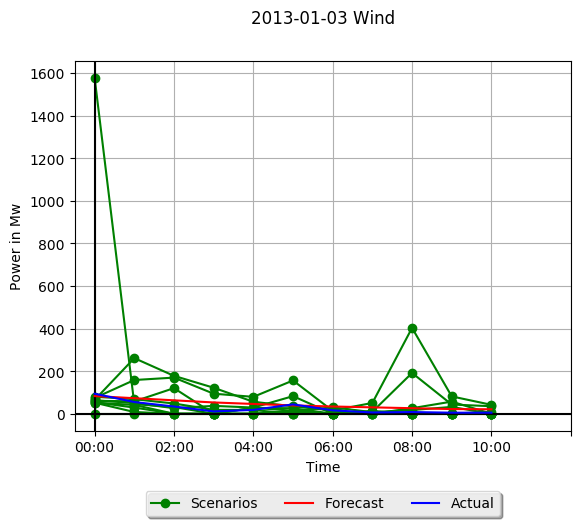
\includegraphics{Wind_example.png}
	\caption{Scenario Plot Produced by \texttt{BPA\_populator\_example.txt}}
	\label{plots}
\end{figure}


\subsubsection{Output}
After executing the script, the user should find a collection of files contained in the \\ \texttt{\$PRESCIENT/examples/gosm\_test/bpa\_output} directory. Within the directory \texttt{pyspdir\_twostage}, the user may find a directory for each day of scenario creation. Within this file will be a collection of structured files with the extension \texttt{.dat} which are used for the purposes of simulation. These files will not be explained here. The raw scenario data will be found in the scenarios.csv file. In the plots directory, there will be a plot of the scenarios themselves as well as of the distributions used to construct the scenarios. The plot of the scenarios is reproduced here in Figure \ref{plots}.

\vspace{50mm}

\section{Formatting Input Files}

With all of the required program dependencies installed, you will now be able to execute various \textit{gosm} scripts to produce and evaluation scenarios. All scripts use generally the same input formats, so it would be useful
to discuss the proper formatting for input files. To use any of the scripts, there are six different types of input files:
\begin{itemize}
	\item options files
	\item data files
	\item sources files
	\item segmentation files
	\item structure files
	\item capacity files
\end{itemize}

Data files are files which contain the raw forecast and actual data for various energy sources as well as the demand for power for a certain set of datetimes.
Sources files are files which specify metadata about the data sources as well as auxiliary information on how to handle the sources.
Segmentation files specify criteria on how to select data which is relevant for a specific datetime being analyzed.
Structure files define the basic structures that are used to create scenarios. Upper bounds files specify an upper threshold to truncate generated scenarios with.
Each of these are explained in further detail in the following sections.
Options files specify controls for how the program as a whole runs and are described above (cf. chapter \ref{sec:options}).

\subsection{Data Files}
Before data can be used by the various \textit{gosm} scripts, it must be processed and formatted in a manner that the programs expect. This process currently entails creating two separate "csv" files for any time-varying data, e.g., load, wind power, or solar power. The first such file contains actual (measured) data and the other contains forecast data. Generally, the forecast data will contain quantities that were predicted day-ahead, and the actuals correspond to the realized quantities. These two files will from now on be referred to as the actuals data file and forecasts data file, respectively. In each of these files, the first column must be labeled as "datetimes" and contain datetime quantities specified in the 'YYYY-MM-DD HH:MM' format; other datetime formats may be recognized as well. The data columns must then be labeled to indicate the type of data quantity being reported -- either "forecasts" or "actuals". You can also have a data file which contains both "forcasts" and "actuals" columns next to each other.

With the newest version of \textit{gosm} we added the option for a planning period length to go through the data in increments of seconds, minutes, hours, etc. Whatever increment you would like to have for the scenario generation process, make sure the data files represent the time step. This means for instance, if your step is 5 hours your data has hourly historic data and if it is 10 minutes your data has historic data for every 10 minutes.

In general, a user will have multiple data files when modeling a single problem, each of which may contain load data, solar generation data, or wind generation data. All such data files must be formatted in the manner described above. An example snippet from a properly formatted data file is as follows:
\begin{figure}[H]
	\begin{framed}
		\noindent
		datetimes,forecasts,actuals\\
		2016-07-01 06:00,160.15, 81\\
		2016-07-01 07:00,710.8, 680\\
		2016-07-01 08:00,1536.78, 1905\\
		2016-07-01 09:00,2103.23, 2113
	\end{framed}
	\caption{Example file structure of a data file}
	\label{fig:structure_data}
\end{figure}



\subsection{Segmentation Files}
For each source of uncertainty, you will need to provide a file for segmentation. Each source can of course be segmented by the same rules as well by providing the same file.
The structure of the file is a series of lines where each line specifies a different criterion to segment the data by. \textit{GOSM} operates by going through each of the lines of the file and sequentially segmenting the data by each criterion. Each line should indicate a segmentation criterion by listing in order the criterion name, column to segment by, type of segmentation, and proportion. 
\bigskip

There are currently two types of segmentation. The first is to segment by window and this will be done if the type is set to \textit{window}. If this method is chosen, then to compute the prediction interval for a given datetime, \textit{GOSM} will select the proportion of points closest to the datetime in the specified field. The other method of segmentation is \textit{enumerate}. This will select all the datetimes which match exactly in the column specified. Note that the cutpoint width is ignored in this method but it still must be provided (can be an arbitrary value). The enumeration method is especially useful if you want to use an external program to segment the data. In this case, you can just use the datetimes found by the external tool to call the segmentation method of \textit{GOSM}.
\bigskip

\begin{figure}[H]
	\begin{framed}
		\lstinputlisting{segment_input.txt}
	\end{framed}
	\caption{Example of a segment criteria file}
	\label{fig:segment}
\end{figure}
%If \textit{PINT} were provided the file shown in Figure \ref{fig:segment}, then it would first segment by forecasts with the \textit{window} method. This means when computing a prediction interval for a certain datetime, it will select the 40\% of points with forecasts closest to the datetime's forecast. Then it will select from this 40\%, the datetimes which have a matching derivative pattern using the \textit{enumerate} method.


\subsection{Structure Files}

Structure files are dat-files including tree template files and scenario template files which specify to the program to construct PySP files for simulation with. These are more complicated structured files which can be better understood with auxiliary sources for the model by which the simulator works.


\subsection{Capacity Files}
If you wish to truncate the values of scenarios by a singular upper bound for certain days, you can specify how to do so with an upper bounds file.
These files are structured to specify an upper bound for a date range, e.g., for the month of August, the power generated must be less than 1000 MW.
To this end, the file will consist of lines in the following format:

\begin{verbatim}
01/01/00, 01/30/00, 20
\end{verbatim}	
This specifies that starting on January 1, and going on until and including January 30, the upper bound is 20. Note that dates are specified in the MM/DD/YY format. Comments are ignored and you may also specify the names of the columns as

\begin{verbatim}
first_date last_date value
\end{verbatim}
before the actual rows with upper bounds, but this is not necessary.

Figure \ref{fig:capacity} shows an actual example of a capacity file.

\begin{figure}[H]
	\begin{framed}
		\lstinputlisting{manual_ub.dat}
	\end{framed}
	\caption{Example of a capacity file}
	\label{fig:capacity}
\end{figure}

\subsection{Sources Files}
To specify all the source-specific information for scenario generation, it is required
that a sources file is written. In this file, all information for every source that is specific
to that source (data files, capacities, source type) must be explicitly defined.

To specify these sources, the user must create a file with \texttt{.txt} extension and within
this file, for every source, write out a Source declaration followed by a parenthesis, then the source's name followed by a comma. 
Then for each source parameter \texttt{key} and the corresponding value \texttt{value}, write \texttt{key="value"} separated by commas.
Note each value must be surrounded by quotation marks. Then terminate the Source with a close parenthesis and a semicolon.
For an example of how this might appear, see Figure \ref{fig:sources}

\begin{figure}[H]
	\begin{framed}
		Source(name1, \\
		key1="value1", \\
		key2="value2" \\
		);\\
		Source(name2,\\
		key1="value3", \\
		key2="value4"\\
		);
	\end{framed}
	\caption{Example sources file}
	\label{fig:sources}
\end{figure}

There are a couple of parameters which must be specified for each source. These are as follows
\begin{itemize}
	\item \textbf{actuals\_file}: The name of the file containing data for actual power generation values. This must have an 'actuals' column. May be the same as the forecasts file.
	\item \textbf{forecasts\_file}: The name of the file containing data for forecasts of power generation.
	This must have a 'forecasts' column. May be the same as the actuals file.
	\item \textbf{source\_type}: The type of source. This is one of 'solar', 'wind', or 'load'.
	\item\textbf{segmentation\_file}: A file containing information about what type of segmentation will be used
	\item\textbf{time\_step}: The time step of the actual and forecast data. The time step must be a 'H' for hours or a 'T' for minutes with an optional prefixed number.
\end{itemize}

In addition to these, there are additional optional parameters that can be specified for each source.
\begin{itemize}
	\item \textbf{capacity\_file}: The name of the file specifying daily capacities for the source.
	\item \textbf{is\_deterministic}: Set to True if the scenario generated from this source should be simply the forecast for the source. Set to False or leave unspecified to have the scenarios generated stochastically.
	\item \textbf{frac\_nondispatch}: The fraction of power which is nondispatchable from this source. This should be a decimal value between 0 and 1.
	\item \textbf{scaling\_factor}: The factor by which to scale the power generation values for this source prior to scenario generation. This should be a decimal value greater than 0.
	\item \textbf{diurnal\_pattern\_file}: A name of the file specifying the diurnal pattern for a given solar source. This may be used to estimate the sunrise and sunset for this source.
	\item \textbf{forecasts\_as\_actuals}: If this options is set to True, then the actuals data will be set to the forecasts data. This option is only allowed if \texttt{is\_deterministic} is also set to True.
\end{itemize}

For an example which sets some of these parameters, see Figure \ref{fig:sources2}
\begin{figure}[H]
	\begin{framed}
		\lstinputlisting{test_sourcelist.txt}
	\end{framed}
	\caption{Real example of a sources file}
	\label{fig:sources2}
\end{figure}

In addition to the above, every sources file must list one source of load data and at least one source of power (either wind or solar).

\section{preprocessor.py}\label{sec:preprocessor}

The preprocessor is a script to prepare the input data files for the scenario creator. It applies thresholds to the power values for each source separately. The user can set a negative and a positive threshold such that all power values greater than the positive threshold are set to this threshold and all values less than the negative threshold are also set to this threshold. This is especially useful for avoiding negative values, which may cause troubles when simulating with the created scenarios.

Running the preprocessor simply requires creating a file which lists all the files you wish to preprocess. 
The format of this file is composed of lines each specifying a file name and the type of source.
An example of this file is in figure \ref{fig:list_of_files.txt}.

\begin{figure}[H]
	\begin{framed}
		\lstinputlisting{list_of_files.txt}
	\end{framed}
	\caption{Example of preprocessor list}
	\label{fig:list_of_files.txt}
\end{figure}

To run preprocessor, use the template for an options file (cf. chapter \ref{sec:template})  and create an options file where$<script>$ would be \texttt{preprocessor.py}. The important $<option>$ variables to consider are \texttt{--preprocessor-list}, which allows one to specify the file with the names of the files to preprocess, and \texttt{--output-directory} where one specifies where to store the preprocessed files. The user also will denote which types of sources to threshold and at what values with the various threshold options listed. An example of this would be \texttt{--wind-power-pos-threshold} and  \texttt{--wind-power-neg-threshold}.

\begin{figure}[H]
	\begin{framed}
		\lstinputlisting{run_preprocessor.txt}
	\end{framed}
	\caption{Example of an options file for preprocessor}
	\label{fig:preprocessor_template_options}
\end{figure}


\section{scenario\_creator.py}\label{sec:scenario_creator}

The script \texttt{scenario\_creator.py} constructs scenarios for a single day of data. The exact algorithm for doing so is described in the following paragraphs.

First, the data is read from the source files. For solar sources, the average hours of sunrise and sunset are estimated for each month in order to discard all data points outside these sunshine hours.

Then the errors (differences between forecasts and actuals) are segmented by the specified segmentation criteria. Then the script calls  \texttt{markov\_populator.py} in order to run the Markov Chain scenario generation process.

In simplified terms the steps in the Markov Chain scenario generation process are:

\begin{itemize}
\item Compute a State Walk from historic data based on a description of a state specified by user arguments
 \item Compute a transition matrix based with probabilities weighted by the frequency with which one state follows another historically
 \item Compute a start state function which chooses a start state by sampling historic states which "match" the data for the date of scenario generation
 \item Generating random walks from a Markov chain with the start state and copulas conditioned on the state before.
 \item Recovering Errors from these walks and then applying them to the forecast of the day and producing scenarios which are then truncated
\end{itemize}

The scenarios can then translated into dat-files as input for a PySP-model. To do so, the user would include in the same directory as \texttt{scenario\_creator.py} a scenario template file and a tree template file. The structure of these files is described in the documentation of \textit{daps}. 
\bigskip

We describe the proper usage of this script using the prior options file (cf. figure \ref{fig:BPA_scenario_creator_example}) as an example. Otherwise using the template for an options file (cf. chapter \ref{sec:template}) , $<script>$ would be \texttt{scenario\_creator.py}. The essential $<option>$ values include:
\begin{itemize}
	\item \textbf{use-markov-chains}: The Markov Chain method is used for generating the scenarios. No value has to be set.
	\item \textbf{copula-random-walk}: Determines if copulas are used for the random walk. Can only be set, if use-markov-chains is also set. For multiple sources, this is a must. No value has to be set.
	\item \textbf{sources-file}: The sourcelist file.
	\item \textbf{output-directory}: The path which stores the output.
	\item \textbf{scenario-template-file}: The scenario template file  used for creating the scenarios. For more information look into the User Manual for Daps.
	\item \textbf{tree-template-file}: The tree template file used for creating the scenarios. For more information look into the User Manual for Daps.
	\item \textbf{reference-model-file}: The reference model which is used for creating the scenarios. For more information look into the User Manual for Daps.
	\item \textbf{scenario-day}: If the scenario creator is run by itself and not by the populator, the scenarios are created for this day only. 
\end{itemize}

Other useful $<option>$ values include: 

\begin{itemize}
	\item \textbf{planning-period-length}: The length of time for the planning or scenario period as an integer directly following by a capital letter, where "H" stands for hours and "T" stands for minutes.
	\item \textbf{number-scenarios}: The number of scenarios generated for each day.
	\item \textbf{error-tolerance}: Used to speed up scenario generation when using three or more sources. This is more of an advanced topic and there is supportive documentation describing this option
	\item \textbf{wind-frac-nondispatch}: A float number.
\end{itemize}

After running the program, the output directory should contain a directory for each date with the desired scenarios in addition to one scenario where forecasts are used and one where actuals are used.

\section{populator.py}

The populator is a simple script which loops over \texttt{scenario\_creator.py} on a specific date range. This is implemented by simply adding options \texttt{--start-date} and \texttt{--end-date} which specify the start and end dates for which you want to compute scenarios. These dates should be provided in YYYY-MM-DD format.
 The option \texttt{--scenario-creator-options-file} is used to specify an options file that is passed to \texttt{scenario\_creator.py} each time it is called. This will come in handy in particular when using the script \texttt{horse\_racer.py} (cf. chapter \ref{sec:horse_racer}). However, those options will be overwritten by the options you explicitly declare in the populator's options file. An example of running \texttt{populator.py} is shown above in the documentation (cf chapter \ref{sec:example}). The essential $<option>$ values include: 
 
 \begin{itemize}
	\item \textbf{start-date \& end-date}: These dates determine the period for which scenarios are created. Both must be in the format of YYYY-MM-DD-HH:MM.
	\item \textbf{output-directory}: The path that stores the output.
	\item \textbf{scenario-creator-options-file}: The options file for the scenario creator.
	\item \textbf{sources-file}: The sourcelist file.
\end{itemize}


\section{horse\_racer.py}\label{sec:horse_racer}

\texttt{horse\_racer.py} is a simple script which links the results from the populator script to the simulator in \textit{prescient}. For the specified sources, it constructs scenarios via
the populator and then uses these scenarios in the simulation specified.
It can be used to specify multiple experiments and the options are to be stored in a configurations file. The options for the populator and the simulator must be specified for each experiment, but either stage can be skipped by passing the option \texttt{--skip}. The format of the configurations file should be as follows:

\begin{verbatim}
	Horse: <name>
	Populator Options:
	<populator options>
	Simulator Options:
	<simulator options>
\end{verbatim}

This format can be repeated as many times as desired in the file. The following file is an example of a configurations file which specifies two experiments.

\begin{framed}
	\lstinputlisting{horse_configurations.txt}
\end{framed}


To execute \texttt{horse\_racer.py}, you must pass two arguments in the command line, the first specifying the configurations file and the second specifying the name of the output file. If no output file is specified, the results are saved in \texttt{results.txt}. For example if we named our configurations file \texttt{horse\_configurations.txt} and wanted to store the results in \texttt{sim\_results.txt}, we would execute the command

\begin{verbatim}
python horse_racer.py horse_configurations.txt sim_results.txt
\end{verbatim}

The final results of the simulation is a collection of stack graphs of the power usage at each day for each of the methods of simulating as well as a csv file containing a summary of the results for the simulation. A sample stack graph is shown in figure \ref{fig:example_stack_graph}.

\begin{figure}[h]
	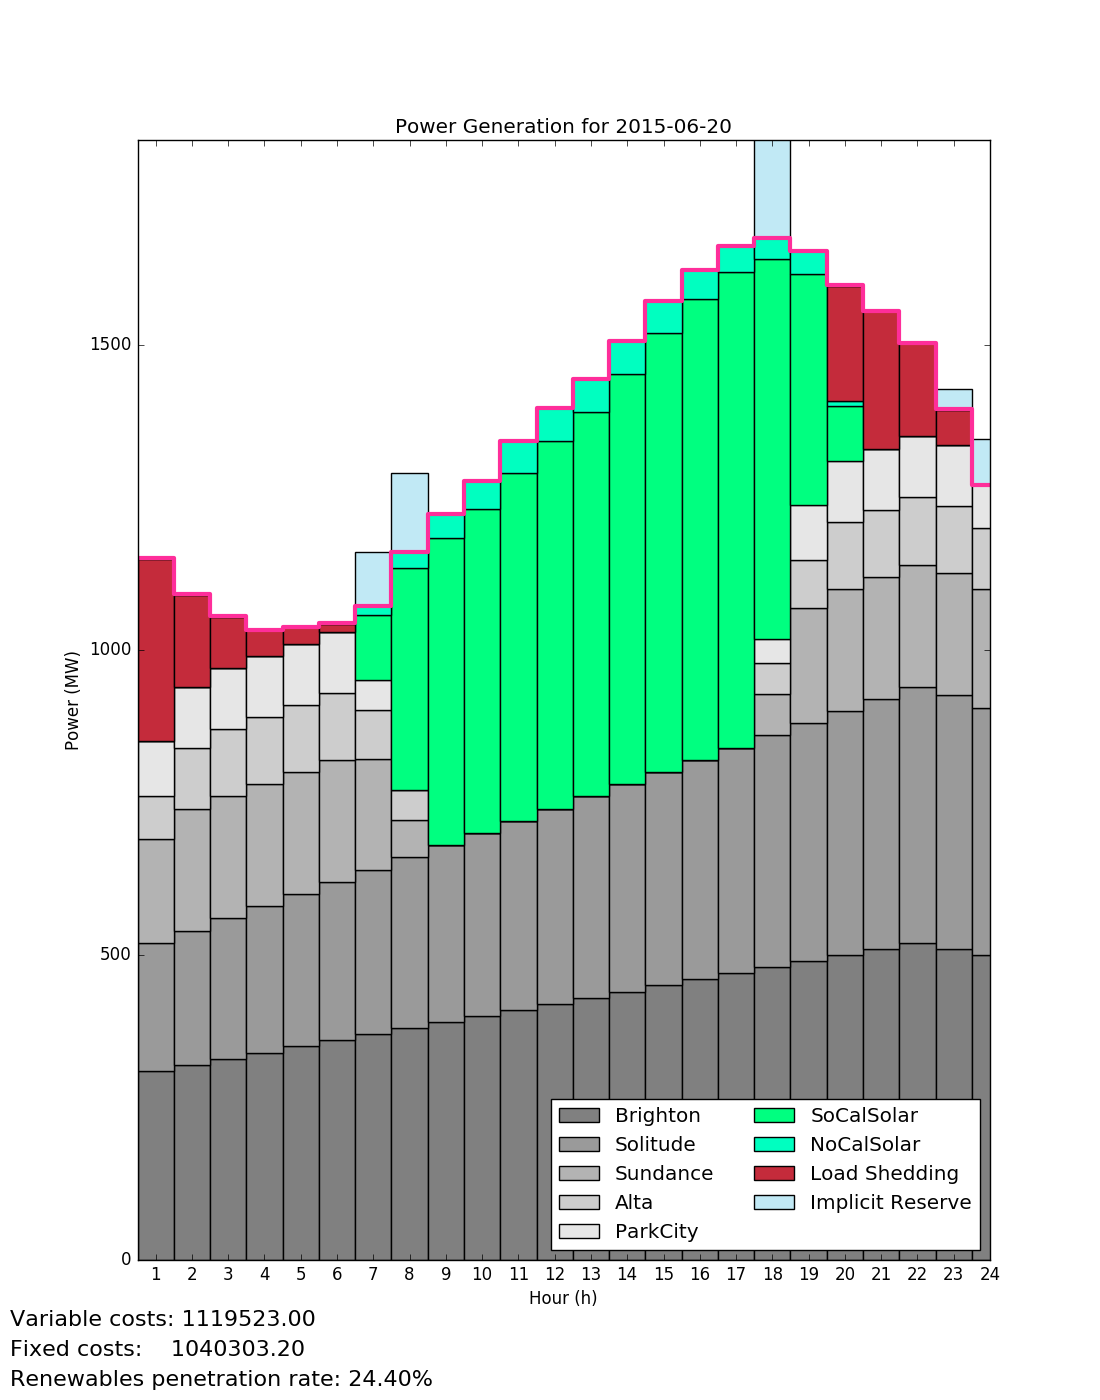
\includegraphics[width=300px]{stackgraph_2015-06-20.png}
	\caption{Example of a stack graph}
	\label{fig:example_stack_graph}
\end{figure}

The csv file produced contains information about the total cost of power generation, load shedding and over generation. The following figure shows an example of this file.

\begin{figure}[H]
	\begin{framed}
		\lstinputlisting{results.txt}
	\end{framed}
	\caption{Example of a result file}
\end{figure}

\iffalse

% This section of advanced topics was in the previous gosm documentation and we are keeping it here just in case it is still needed

\section{Advanced Topics}

\subsection{Spatial Copulas}
If the user wishes to take into account dependencies across space when constructing scenarios, he or she will want to use spatial copulas. This can be done by specifying the  \texttt{--use-spatial-copula} option and a partition file with the \texttt{--partition-file} option. 

For an example of how the scenario creator options file should be structured, see Figure \ref{spatial}. We note that the user can specify a specific copula which can be fit with the \texttt{--spatial-copula} option, of which currently only the Gaussian Copula is available as an option. The user can also specify the \texttt{--use-same-paths-across-correlated-sources} which means that for a specific scenario, on each of the correlated sources, the same hyperrectangle set will be used. For uncorrelated sources, different sources may use different hyperrectangles.

\begin{figure}
	\begin{framed}
	\lstinputlisting{spatial.txt}
	\end{framed}
	\caption{An example scenario creator file for spatial copulas}
	\label{spatial}
\end{figure}

\subsubsection{Partition Files}
For the purposes of using spatial copulas, it is necessary to specify which
sources are related. For \textit{GOSM}, this is done using a partition file.
In it, sources which are related are grouped together and any singleton source
is specified in its own section.

The structure of the file is as follows:
\begin{verbatim}
<Group1 Name>:
-<Source1>
-<Source2>
...

<GroupN Name>:
-<SourceN1>
-<SourceN2>
...
Singletons:
-<SingleSource1>:
-<SingleSource2>:
\end{verbatim}

For good measure, an actual partition file example is in Figure \ref{fig:partition}.

\begin{figure}[H]
	\begin{framed}
		\lstinputlisting{partition.txt}
	\end{framed}
	\caption{Example of a partition file}
	\label{fig:partition}
\end{figure}

\subsection{Disaggregated Sources}
In certain circumstances, it may be the case that a user has a source which is actually an aggregation of multiple sources. This user may want to generate scenarios using this aggregate source and then have the generated scenarios be disaggregated according to certain proportions. This can be done by setting the "aggregate" option for a given source to "True" and then setting the "disaggregation\_file" to a file which has the following format:

\begin{verbatim}
source,proportion
<Source1>,<Proportion1>
<Source2>,<Proportion2>
...
\end{verbatim}
In the above, \texttt{<Source1>} refers to the name of the first component source of the aggregate source and \texttt{<Proportion1>} is the corresponding proportion of the power which the source should be producing.

An example of this disaggregation file is presented in Figure \ref{fig:disaggregation}.
\begin{figure}[H]
	\begin{framed}
		\lstinputlisting{wind_generators.txt}
	\end{framed}
	\caption{Example of a disaggregation file}
	\label{fig:disaggregation}
\end{figure}

A sources file which might appear with this disaggregation file is also shown in Figure \ref{fig:disaggregation-sources}.
\begin{figure}[H]
	\begin{framed}
		\lstinputlisting{bpa_sourcelist_aggregate.txt}
	\end{framed}
	\caption{Example of a disaggregation file}
	\label{fig:disaggregation-sources}
\end{figure}

\fi
\end{document}
